\documentclass[11pt]{article}
\usepackage[margin=0.9in]{geometry}
\usepackage{amsmath,amssymb}
\usepackage{booktabs}
\usepackage{enumitem}
\usepackage{tikz}
\usetikzlibrary{positioning}
\usepackage[hidelinks]{hyperref}
\setlist{nosep,leftmargin=1.4em}
\setlength{\parskip}{3pt}
\setlength{\parindent}{0pt}

\title{\vspace{-1.5em}Certified Conditional Cooperation Between Programs:\\ What We Tried, What We Learned, and When to Return}
\author{Findings memo for Cam and collaborators \quad (\texttt{\~{}/dev/diag}, November 2026)}
\date{\vspace{-2.5em}}

\begin{document}
\maketitle

\begin{center}
\fbox{\parbox{0.94\linewidth}{\small
\textbf{Status: parked.} We built a machine-checked scheme in which programs cooperate in the Prisoner's Dilemma by exchanging proof certificates, and it works. But the guarantees it provides turn out to depend on an assumption that the whole program-equilibrium literature makes implicitly: a \emph{binding executor} that runs the code each player shows and delivers both moves. With such an executor, a plain escrow contract already provides our guarantees; without one, no scheme can provide them exactly. Our approach would matter only in a setting with binding execution but no shared contract, where each agent keeps its own code. We could not name one. \emph{Return if someone can} (see the table at the end).}}
\end{center}

\section*{1\quad The goal}

Open-source game theory studies agents that can read each other's source code before acting. In the one-shot Prisoner's Dilemma (payoffs $T > R > P > S$ for temptation, reward, punishment and sucker), this allows \emph{conditional} cooperation. The best-known example is FairBot, which cooperates if it can prove that its opponent cooperates with it. By Löb's theorem, two FairBots cooperate, even if they are written differently. However, FairBot must \emph{search} for that proof. Exhaustive search over proofs of length $B$ costs about $|\Sigma|^B$, which is affordable only up to $B \approx 20$--$28$, while Critch's bounded version of the argument needs proofs of length $B \gtrsim 10^4$.

Our idea was to replace search with checking, as in proof-carrying code. Players agree in advance on a \emph{standard} $K$. Each player submits its program together with a \emph{certificate}: a proof that the program satisfies $K$. An LLM writes both, and at play time each side runs a single certificate check.

\section*{2\quad What we built}

The difficulty is self-reference: $K$ must say ``I cooperate with you exactly when your certificate proves that \emph{you} satisfy $K$''. Naive versions either regress (a proof about a proof about\ldots) or fall into the \emph{Löb trap}, where letting the logic reason about its own checker makes every program a member, DefectBot included. We avoid both. We define $K$ with the diagonal lemma rather than Löb's theorem, and we give the object logic $S$ no reflection rule about its own checker.

Everything is formalized in Lean~4 with no \texttt{sorry} and only Lean's three standard axioms.\footnote{The DSL, its fuel-bounded interpreter \texttt{run} (each operation is charged the size of the value it builds, so values stay bounded by fuel: \texttt{eval\_sz\_le}), the logic $S$ with checker \texttt{check} (soundness: \texttt{check\_sound}), and the theorems \texttt{theoremA}, \texttt{theoremB}, \texttt{exclusivity}. CertBot's certification and tournament outcomes are kernel-checked with \texttt{unseal} and \texttt{decide +kernel}, with no \texttt{native\_decide} or \texttt{\#eval}. Progress log: \texttt{PROGRESS.md}.} We prove that the checker is sound, and two theorems about the standard: two certified members cooperate (Theorem~A), and a certified member is never exploited (Theorem~B). A one-way variant $K'$ and an exclusivity theorem show that the standards are \emph{closed}: no program satisfies both $K$ and $K'$, and a $K$-member and a $K'$-member defect against each other even though both are ``cooperative''. Certificates have 1.7k--50k nodes and a game takes about 5\,ms. In a pilot, an LLM wrote 8 of 8 members correctly (6 on the first attempt), and the checker rejected all 6 adversarial attempts. The generator was the same model that built the system, so this is not independent evidence.

The construction works. What it does not yet have is a reason why anyone needs it.

\section*{3\quad What we found}

\textbf{Necessity does not single out certificates.} We first tried to show that the approach is forced: if P $\neq$ NP, no fast agent is both \emph{fair} (cooperates whenever a short proof of the opponent's cooperation exists) and \emph{unexploitable}. Our Lean version assumed its two hard steps as hypotheses, and with a fixed fuel cap one of them is false for large inputs. More importantly, a much simpler diagonal argument already gives the conclusion unconditionally. Using Contrarian, which plays the opposite of whatever you play against it, one shows that no agent whose runs have short proofs is both fair and unexploitable, with no P $\neq$ NP assumption and no induction. This argument is folklore-level (Anderlini 1990; Barasz et al., \S5), and it constrains \emph{every} feasible approach, so it cannot argue for ours.

\textbf{Zero exploitability is not a requirement.} Since necessity cannot justify our criteria, the criteria must justify themselves, and unexploitability does not. Oesterheld's $\varepsilon$-grounded FairBot, which cooperates unconditionally with probability $\varepsilon$, is already an equilibrium: defecting against it earns about $\varepsilon T + (1-\varepsilon)P < R$ for small $\varepsilon$. The claim therefore narrows to what Theorems A and B actually say together: a \emph{verifiable conditional commitment}, ``I cooperate if and only if you make the same commitment''.

\textbf{That commitment depends on an executor.} Note that Theorems A and B, like every program-equilibrium result we know of, assume that the code each player shows is the code that runs and that both moves are delivered. Making this assumption explicit splits the problem in two (Figure~\ref{fig:executor}). \emph{With} a binding executor, such as a smart contract or a referee, a plain escrow contract (``both commit, then both cooperate'') already gives A and B; this is Monderer and Tennenholtz's mediator. \emph{Without} one, consider the following attack. Certified agent $b$ blocks its own incoming channel. It never receives $a$'s certificate, so it defects, and it does so ``honestly'', exactly as $K$ prescribes. Meanwhile $a$ receives $b$'s certificate and cooperates, so $a$ is exploited. Signed receipts only move the problem one level up. This is the fair-exchange impossibility (Even and Yacobi; Pagnia and Gärtner) in strategic form. Its known escapes, collateral and gradual release, cost some $\varepsilon$ of exploitability, which is the same price $\varepsilon$-grounding already pays.

\begin{figure}[h]
\centering
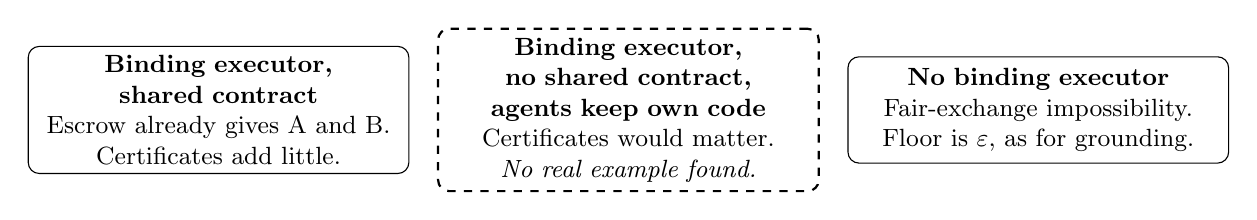
\begin{tikzpicture}[box/.style={draw,rounded corners,align=center,font=\small,text width=4.6cm,minimum height=1.35cm}]
\node[box] (a) {\textbf{Binding executor, shared contract}\\ Escrow already gives A and B.\\ Certificates add little.};
\node[box,right=0.35cm of a,dashed,thick] (b) {\textbf{Binding executor, no shared contract, agents keep own code}\\ Certificates would matter.\\ \emph{No real example found.}};
\node[box,right=0.35cm of b] (c) {\textbf{No binding executor}\\ Fair-exchange impossibility.\\ Floor is $\varepsilon$, as for grounding.};
\end{tikzpicture}
\caption{Where certificate-based cooperation could matter. Only the dashed middle regime distinguishes our approach, and we could not populate it.}
\label{fig:executor}
\end{figure}

\section*{4\quad The open question}

Our one distinctive feature is \emph{semantic membership}: any program that is \emph{proved} to honor $K$ is a member, rather than one exact program (CliqueBot) or one escrow address. That feature matters only in the middle regime of Figure~\ref{fig:executor}. The bare program-equilibrium model belongs there by definition, but it is a model, not a deployment. The most plausible real candidate, which we have not examined, is hardware-governance commitments of the flexHEG kind (``if the other party makes the same commitment''). In hindsight, most of our effort (the necessity theorem, about 135 literature searches) went to questions that do not bear on this one.

\section*{5\quad Paths to a paper}

\textbf{The hidden-assumption paper.} The executor finding is itself the most promising result. Program-equilibrium results silently assume a binding runner. Making that explicit shows that unexploitable conditional cooperation \emph{is} fair exchange: with an executor, escrow suffices; without one, $\varepsilon$ is the floor. Critch, Oesterheld and our certificates are then points on one map. The cooperative-AI literature lists checkable conditional commitments as an open problem (for example, DiGiovanni, Clifton and Macé 2025 leave template checking to future work), so this audience may not know the reduction. The risk is that cryptographers consider it folklore. Our searches found no written version, but they were snippet-level and confabulated at least one source, so that is weak evidence.

\textbf{A theory note} for open-source game theory: shipped proofs plus the diagonal lemma give cooperation with no proof search and no Löb, all machine-checked. It is modest, and the artifact already exists. The closest work we verified is Duclaux et al.\ 2026 (offline Lean proofs of outcomes for each pair of bots) and Ondras 2026 (a Lean handshake with a trusted attestation step).

\textbf{A full paper on the construction} only if the middle regime turns out to be real. It would then also need an LLM run with an independent model, and an answer to interoperation between different standards.

\section*{6\quad When to pick this up}

\begin{center}
\small
\begin{tabular}{@{}p{0.40\linewidth}p{0.55\linewidth}@{}}
\toprule
\textbf{Resume if\ldots} & \textbf{Cheapest test} \\
\midrule
A real setting has binding execution but no shared contract, and agents keep their own code & Spend 30 minutes trying to name one, starting with flexHEG. Then check whether a single ``CliqueBot-as-escrow'' contract emulates it; if so, the case fails. \\
Nobody has written ``program equilibrium = fair exchange'' & One hour of searching with opened sources only (Harrenstein 2007; Katz 1991; rational fair exchange), and one email to Oesterheld or DiGiovanni. \\
Someone has a real use for template checking & Ask DiGiovanni, Clifton and Macé what they intended it for. \\
\midrule
\multicolumn{2}{@{}p{0.96\linewidth}@{}}{\textbf{Stop if} the reduction is already known \emph{and} no middle-regime setting turns up. Then archive the Lean repository and post, at most, a short note.}\\
\bottomrule
\end{tabular}
\end{center}

If we do return, ask first what the criteria are and whether an executor is assumed, before proving theorems. Treat any literature claim without an opened source as unverified. The Lean development, the literature corpus (about 110 reports, in \texttt{research/related\_work/}) and the record of hypotheses tried (\texttt{research/OUTLINE\_2026-11-18.md}) are reusable whatever we decide.

\end{document}
